
%
% Note that the a4paper option is mainly intended so that authors in
% countries using A4 can easily print to A4 and see how their papers will
% look in print - the typesetting of the document will not typically be
% affected with changes in paper size (but the bottom and side margins will).
% Use the testflow package mentioned above to verify correct handling of
% both paper sizes by the user's LaTeX system.
%
% Also note that the "draftcls" or "draftclsnofoot", not "draft", option
% should be used if it is desired that the figures are to be displayed in
% draft mode.
%
%\documentclass[journal,draftcls,onecolumn,12pt,twoside]{IEEEtranTCOM}
\documentclass[journal,twoside]{IEEEtranTCOM}
%


\normalsize


\usepackage[dvips]{graphicx}

\usepackage[cmex10]{amsmath}
%\usepackage{dsfont}

\usepackage{algorithm}
\usepackage{algpseudocode}

\usepackage{amssymb}
\usepackage{multirow}
%\usepackage{multicol}

\usepackage{cite}

\begin{document}
%
% paper title
% can use linebreaks \\ within to get better formatting as desired
\title{A User Selection Algorithm Using Angle between Subspaces for Downlink MU-MIMO Systems }
%
%
% author names and IEEE memberships
% note positions of commas and nonbreaking spaces ( ~ ) LaTeX will not break
% a structure at a ~ so this keeps an author's name from being broken across
% two lines.
% use \thanks{} to gain access to the first footnote area
% a separate \thanks must be used for each paragraph as LaTeX2e's \thanks
% was not built to handle multiple paragraphs
%

\author{Seongho~Nam,
        Jeongchan~Kim,
        and~Youngnam~Han,~\IEEEmembership{Senior Member,~IEEE}
\thanks{This research was funded by the MSIP(Ministry of Science, ICT \& Future Planning), Korea in the ICT R\&D Program 2013.

S. Nam, J. Kim and Y. Han are with the Department
of Electrical Engineering, Korea Advanced Institute of Science and Technology (KAIST), Republic of Korea (e-mail: \{indnd, monirer, ynhan\}@kaist.ac.kr). }

}


% The paper headers
\markboth{IEEE Transactions on Communications}%
{Revised paper}
% The only time the second header will appear is for the odd numbered pages
% after the title page when using the twoside option.
%
% *** Note that you probably will NOT want to include the author's ***
% *** name in the headers of peer review papers.                   ***
% You can use \ifCLASSOPTIONpeerreview for conditional compilation here if
% you desire.




% If you want to put a publisher's ID mark on the page you can do it like
% this:
%\IEEEpubid{0000--0000/00\$00.00~\copyright~2007 IEEE}
% Remember, if you use this you must call \IEEEpubidadjcol in the second
% column for its text to clear the IEEEpubid mark.





\maketitle


\begin{abstract}
One of major issues in the efficient use of radio resource for multiuser multiple-input/multiple-output (MU-MIMO) systems is the selection of users to achieve the maximum system throughput.  The optimal user selection algorithm, which requires exhaustive search, is prohibitive due to its high computational complexity where Block diagonalization (BD) method is applied and known as a suboptimal precoding technique for downlink MU-MIMO  systems, which intents to perfectly eliminate inter-user interference. In this paper, we propose  efficient, iterative user selection algorithms with low complexity, where the product of eigenvalues of effective channels is utilized as a selection metric by applying the concept of principal angles between subspaces. And, we further examined the applicability of  the proposed algorithms to limited feedback systems and proportional fair (PF) scheduling. Through computational complexity analysis, we show that the proposed algorithm has low complexity with a little loss in throughput. Simulation results validate that the proposed algorithm achieves almost the same system throughput by a capacity-based algorithm under high SNR regime with considerable reduction in complexity.
\end{abstract}

% Note that keywords are not normally used for peerreview papers.
\begin{IEEEkeywords}
Multiuser multiple input multiple output (MU-MIMO), user selection, principal angle, proportional fairness (PF), limited feedabck
\end{IEEEkeywords}






% For peer review papers, you can put extra information on the cover
% page as needed:
% \ifCLASSOPTIONpeerreview
% \begin{center} \bfseries EDICS Category: 3-BBND \end{center}
% \fi
%
% For peerreview papers, this IEEEtran command inserts a page break and
% creates the second title. It will be ignored for other modes.
\IEEEpeerreviewmaketitle




\section{Introduction} \label{Section:Introduction}
\IEEEPARstart{M}{ulti-user} multiple-input/multiple-output (MU-MIMO) systems have drawn huge amount of attention recently due to their capability to enhance system capacity. For a downlink MU-MIMO system, it is widely known that dirty paper coding (DPC) \cite{DPC} can achieve the capacity region, but it requires tremendous computational complexity for successive encoding and decoding. In order to avoid the complexity of DPC, practical precoding techniques have been proposed using  zero-forcing beamforming (ZF-BF) and  block diagonalization (BD) are posed. A ZF-BF is proposed for the multiple-input/single-output (MISO) systems \cite{ZF1,ZF2}, where ZF-BF eliminates inter-user interference by designing a precoding matrix as the pseudo-inverse of selected users' channels. For the case when users have multiple receive antennas, BD method is introduced \cite{BD}. BD can eliminate inter-user interference totally by a well designed precoding matrix to lie in the null space of all other users' channel matrices. With BD, an MU-MIMO channel can be decomposed into a complying number of parallel single-user MIMO (SU-MIMO) channels.

Under the constraint that a precoding matrix lies in the null space of the other user's channel matrices, the number of users that can be simultaneously served by a base station (BS) is limited by the number of transmit antennas and receive antennas. Typically when the total number of users in a system is much larger than the maximum number of supportable users, a BS is required to select a set of users to maximize data rate. The optimal user set can be obtained by searching over all possible subsets of users, but it requires prohibitively heavy computational burden.

In order to reduce the user selection complexity under BD schemes, a lot of research has been conducted on reducing the complexity in designing a precoder.
In the traditional singular value decomposition (SVD)-based  precoder design method, frequent SVDs are required for finding a precoding matrix causing high complexity. To avoid the frequent SVD, an iterative precoder design method is proposed in \cite{SRN}. And for the optimal user selection, many greedy algorithms to select one user that maximizes selection metric at each iteration have been proposed to reduce the complexity. A capacity-based suboptimal user selection algorithm (c-algorithm) is proposed in \cite{c_n}, which iteratively selects a user to maximize system capacity from a set of  unselected users, but it requires a large amount of SVD operations to obtain precoding matrices. To reduce the complexity, various user selection metrics are proposed such as Frobenius norm, determinant, correlation, chordal-distance, and etc. \cite{c_n,Determinant,Correlation1,Correlation2,CD_conf,CD_jour}. %A Frobenius norm based algorithm (n-algorithm) selects a user based on the Frobenius norm of an effective channel matrix, whose complexity is lower than c-algorithm. From the fact that the determinant can be used as a measure of orthogonality as well as channel quality, a determinant-based user selection algorithm is proposed \cite{Determinant}. In \cite{Correlation1,Correlation2}, the correlation-based user selection algorithms are proposed and algorithms based on a chordal distance metric which is measured by the angle between channel matrices are proposed in \cite{CD_conf,CD_jour}.
These low complexity user selection algorithms can reduce the computational burden, but performance degradation is inevitable.

In addition, these low complex user selection algorithms cannot consider the issue of fairness. Note that since the selection metric of conventional algorithms except c-algorithm is not the data rate, these user selection algorithms cannot be applied to proportional fairness (PF) scheduling. The product of squared row norms of the effective channels is proposed as a user selection metric for the PF scheduling \cite{SRN}. This method is motivated by the relationship between the eigenvalues and row norms of a Hermitian matrix, which provides low complexity with reasonable performance, and can be easily modified for PF scheduling.

In this paper, we propose a low-complexity user selection algorithm for a different metric, the product of eigenvalues of effective channel matrices from angle between subspaces. Through the recursive derivation of the metric. the proposed method can effectively reduce the complexity in user selection where the product of eigenvalues can be obtained from that of the previous iteration recursively using the relationship between principal angles and eigenvalues.
And, we show that  the lower bound on the product of eigenvalues can be used as a simplified selection metric. The proposed algorithm can be directly applicable to PF scheduling and a system with limited feedback scenario, where each user feeds back partial channel state information (CSI)  of direction and quality. Simulation results show that the proposed algorithm outperforms other low complex user selection algorithms in high SNR regime, and especially achieves almost the same sum rate as c-algorithm.  A similar research which utilizes an angle between subspaces is proposed with different metric in \cite{Algo:Subspace}.


The rest of this paper is organized as follows. The  downlink MU-MIMO system model is described in Section \ref{Section:SystemModel}. We propose a low complex user selection algorithm in Section \ref{Section:Algorithm}. In Section \ref{Sec:PracticalIssues}, we consider the practical applications of our algorithm to  proportional fairness scheduling and the systems of limited feedback. Simulation results are provided in Section \ref{Section:Simulation Results} and conclusions are drawn in Section \ref{Section:Conclustion}.

\textit{Notation}: Bold uppercase and lowercase letters represent matrices and vectors, respectively. The conjugate transpose of a matrix and the transpose of a matrix is denoted by $(\cdot)^*$ and $(\cdot)^T$, respectively. $\cal{R}({\bf{H}})$ and $\cal{N}({\bf{H}})$ represent the row space and the null space of ${\bf{H}}$, respectively. Furthermore, $\mathrm{row}({\bf{H}})$ and $\mathrm{null}({\bf{H}})$ denote the matrices whose columns form an orthonormal basis of $\cal{R}({\bf{H}})$ and $\cal{N}({\bf{H}})$, respectively.

\section{System Model} \label{Section:SystemModel}
Consider a downlink MU-MIMO system with one BS and $K$ users. The BS has $n_t$ transmit antennas and each user has the same number of receive antennas $n_r$. We assume that the channel is quasi-static so that the channel is constant during one scheduling interval, and varies randomly over the interval.

Let ${\cal{S}} \subset \{1,2,\cdots,K\}$ denote a set of users to be simultaneously supported by a BS over the co-channels. And ${\bf{x}}_k \subset {\mathbb{C}}^{n_r \times 1}$ denotes transmitted signal vector for the $k$-th user. For the simplicity of our analysis, we assume that $n_r$ data streams are transmitted to each user. The BS transmits ${\bf{x}}_k$ multiplied by its precoding matrix ${\bf{T}}_k  \subset {\mathbb{C}}^{n_t \times n_r}$, so that the signal vector transmitted from the BS can be described as

\begin{equation} \label{eq:TransmittedSignal}
{\bf{x}} = \sum\limits_{k = 1}^{\left| \cal{S} \right|} {{{\bf{T}}_k}{{\bf{x}}_k}},
\end{equation}
where ${\left| \cal{S} \right|}$ denotes the cardinality of $\cal{S}$.
So, the received signal at the $k$-th user is given by
\begin{eqnarray} \label{eq:received signal}
{{\bf{y}}_k} &  = & {{\bf{H}}_k}{\bf{x}} + {{\bf{n}}_k}  \nonumber \\
& = & {{\bf{H}}_k}{{\bf{T}}_k}{{\bf{x}}_k} + \sum\limits_{j \ne k} {{{\bf{H}}_k}{{\bf{T}}_j}{{\bf{x}}_j}}  + {{\bf{n}}_k},
\end{eqnarray}
where ${\bf{H}}_k \subset {\mathbb{C}}^{n_r \times n_t}$ is the complex channel matrix from the BS to the $k$-th user with each element distributed by independently and identically distributed (i.i.d.) complex Gaussian distribution ${\mathcal{CN}}(0,1)$ and ${\bf{n}}_k \subset {\mathbb{C}}^{n_r \times 1}$ is the additive white complex-Gaussian noise vector with zero mean and covariance matrix ${\bf{I}}_{n_r}$. For analytical simplicity, we assume that $n_t>n_r$ and $\mathrm{rank}({\bf{H}}_k)=\mathrm{min}(n_r,n_t)=n_r$.

The basic idea of BD is to nullify inter-user interference. For zero-interference constraint, a precoding matrix ${\bf{T}}_j$ for user $j$ is designed such that
\begin{equation} \label{eq:precoder constraint}
{{\bf{H}}_k}{{\bf{T}}_j} = 0,\forall k \ne j.
\end{equation}

The precoding matrix ${{\bf{T}}_k}$ can be decomposed into two matrices ${\bf{Z}}_k$ and ${\bf{B}}_k$, i.e., ${{\bf{T}}_k}={\bf{Z}}_k{\bf{B}}_k$, where ${\bf{Z}}_k$ is designed to eliminate inter-user interference and ${\bf{B}}_k$ is designed to maximize the data rate. For that, ${\bf{Z}}_k$ should lie in ${\cal{N}}({\bf{\tilde H}}_k)$ to eliminate inter-user interferences, where ${\bf{\tilde H}}_k$ is the aggregate channel matrix of the other users, i.e.,
\begin{equation} \label{eq:H_tilde}
{{{\bf{\tilde H}}}_k} = {[{\bf{H}}_1^T\, \cdots \,\,{\bf{H}}_{k - 1}^T\,{\bf{H}}_{k + 1}^T\, \cdots \,\,{\bf{H}}_{\left| \cal{S} \right|}^T]^T}.
\end{equation}

%There are two ways to obtain ${\bf{Z}}_k$: singular value decomposition (SVD)-based approach \cite{BD} and iterative approach \cite{SRN}. The SVD-based approach is to find ${\bf{Z}}_k$ by applying SVD over ${\bf{\tilde H}}_k$. ${\bf{\tilde H}}_k$ is decomposed by SVD as follows:
%
%\begin{equation} \label{eq:SVD H_tilde}
%{{{\bf{\tilde H}}}_k} = {{{\bf{\tilde U}}}_k}[{{{\bf{\tilde \Sigma }}}_k} \, {\bf{0}}]{[{\bf{\tilde V}}_k^{(1)} \, {\bf{\tilde V}}_k^{(0)}]^*},
%\end{equation}
%where ${\bf{\tilde V}}_k^{(0)}$ forms a basis of ${\cal{N}}({\bf{\tilde H}}_k)$. Thus, ${\bf{Z}}_k$ is simply obtained as ${\bf{Z}}_k={\bf{\tilde V}}_k^{(0)}$.

${\bf{Z}}_k$ is obtained by an iterative approach \cite{SRN}, recursively. Let ${\bf{Z}}_k^{(i)}$ be ${\bf{Z}}_k$ at the $i$-th iteration. Without loss of generality, we describe an iterative precoder design method for only the first user. At the initial step, we set ${\bf{Z}}^{(1)}_1=\bf{I}$. At the $i$-th iteration, since ${\bf{Z}}^{(i)}_1$ should satisfy that ${{\bf{H}}_k}{\bf{Z}}^{(i)}_1=0$ for all $1 < k \leq i$, ${\bf{Z}}^{(i)}_1$ can be obtained recursively from ${\bf{Z}}^{(i-1)}_1$ as follows:
\begin{equation}
{\bf{Z}}^{(i)}_1={\bf{Z}}^{(i-1)}_1 {{\bf{G}}_1^{(i)}},
\end{equation}
where ${{\bf{G}}_1^{(i)}}$ lies in ${\cal{N}}\left({\bf{H}}_{i}{\bf{Z}}^{(i-1)}_1\right)$. We can simply select ${\bf{G}}_1^{(i)}=\mathrm{null}\left({\bf{H}}_{i}{\bf{Z}}^{(i-1)}_1\right)$. Similarly, the precoding matrices of other users can be obtained recursively. %The complexity of the iterative approach is known to be lower than that of SVD-based method \cite{SRN}. Moreover, since this iterative method conforms to greedy user selection algorithms, an iterative approach is taken for finding a precoding matrix.

The zero-interference constraint is met by a precoding, and an MU-MIMO channel is decomposed into a set of equivalent parallel SU-MIMO channels by BD. Let ${\bf{\bar H}}_k$ denote the effective channel matrix of the $k$-th user, i.e., ${{{\bf{\bar H}}}_k} = {{\bf{H}}_k}{{\bf{Z}}_k}$. To complete precoder design, we should find ${{\bf{B}}_k}$ to maximize data rate. We can denote the SVD of ${{{\bf{\bar H}}}_k}$ as
\begin{equation}
{{{\bf{\bar H}}}_k}={{{\bf{\bar U}}}_k}[{{\bf{\bar \Sigma}}_k} \,  {\bf{0}}] {[{\bf{\bar V}}_k^{(1)} \, {\bf{\bar V}}_k^{(0)}]^*},
\end{equation}
where ${{{\bf{\bar V}}}^{(1)}_k}$ holds the first $n_r$ right singular vectors. In order to maximize data rate, we set ${{\bf{B}}_k}={{{\bf{\bar V}}}^{(1)}_k}$. Note that the columns of ${{\bf{B}}_k}$ correspond to the orthonormal basis of ${\cal{R}}({{{\bf{\bar H}}}_k})$, i.e., ${{\bf{B}}_k}=\mathrm{row}({{{\bf{\bar H}}}_k})$.


%The zero-interference constraint is met by precoding, and an MU-MIMO channel is decomposed into a set of equivalent parallel SU-MIMO channels by BD. Let ${\bf{\bar H}}_k$ denote the effective channel matrix of the $k$-th user, i.e., ${{{\bf{\bar H}}}_k} = {{\bf{H}}_k}{{\bf{Z}}_k}$. To complete precoder design, we should find ${{\bf{B}}_k}$ to maximize data rate. The sum rate of BD under a total power constraint $P$ is given by
%\begin{equation} \label{eq:SumRate}
%R({\cal{S}}) = \mathop {\max }\limits_{{{\bf{B}}_k},{{\bf{Q}}_k}:\sum\nolimits_{k = 1}^{\left| {\cal{S}} \right|} {\mathrm{Tr}({{\bf{Q}}_k})}  \le P} \sum\limits_{k = 1}^{\left| {\cal{S}} \right|} {{{\log }_2}\det \left({\bf{I}} + {{{\bf{\bar H}}}_k}{{\bf{B}}_k}{{\bf{Q}}_k}{{\bf{B}}^*_k}{\bf{\bar H}}_k^*\right)},
%\end{equation}
%where ${{\bf{Q}}_k}=E[{{\bf{x}}_k}{\bf{x}}_k^*]$ is the covariance matrix of the $k$-th user and $P$ is total transmit power. The optimal solution of (\ref{eq:SumRate}) is to let ${{\bf{B}}_k}$ be the right singular vectors of ${{{\bf{\bar H}}}_k}$ with optimal power loading \cite{BD}. Since we can denote the SVD of ${{{\bf{\bar H}}}_k}$ as
%\begin{equation}
%{{{\bf{\bar H}}}_k}={{{\bf{\bar U}}}_k}[{{\bf{\bar \Sigma}}_k} \,  {\bf{0}}] {[{\bf{\bar V}}_k^{(1)} \, {\bf{\bar V}}_k^{(0)}]^*},
%\end{equation}
%where ${{{\bf{\bar V}}}^{(1)}_k}$ holds the first $n_r$ right singular vectors, we can simply choose ${{\bf{B}}_k}={{{\bf{\bar V}}}^{(1)}_k}$. Note that the columns of ${{\bf{B}}_k}$ correspond to the orthonormal basis of ${\cal{R}}({{{\bf{\bar H}}}_k})$, i.e., ${{\bf{B}}_k}=\mathrm{row}({{{\bf{\bar H}}}_k})$. The optimal power loading coefficients are obtained by the water-filling algorithm over the eigenvalues of $\{ {{{\bf{\bar H}}}_k}{\bf{\bar H}}_k^*\} _{k = 1}^{\left| {\cal{S}} \right|}$, which correspond to diagonal entries of ${{{\bf{\bar \Sigma}}}^2_k}$.


Note that the number of the transmit antennas has to be larger than the sum of the number of receive antennas of the other users for the existence of the null space of ${\bf{\tilde H}}_k$, i.e.,
\begin{equation} \label{eq:Kmax constraint}
{n_t>(|\mathcal{S}|-1)n_r}.
\end{equation}

From (\ref{eq:Kmax constraint}), the maximum number of simultaneously supportable user $\hat{K}$ is limited by $\lceil \frac{{{n_t}}}{{{n_r}}} \rceil$, where $\lceil x \rceil$ is the ceiling function. When $K$ is large, constructing a set of supportable users, $\cal{S}$ is very critical to maximize overall throughput. The optimal user set is found by searching over all possible subsets as follows:
%\begin{equation} \label{eq:OptUserSet}
%{{\mathcal{S}}^*} = \mathop {\arg \max }\limits_{{\mathcal{S}} \subset \{ 1,2, \cdots ,K\} \atop | {\mathcal{S}} | \le \hat K} R({\mathcal{S}}).
%\end{equation}
\begin{equation} \label{eq:OptUserSet}
{{\mathcal{S}}^*} = \mathop {\arg \max }\limits_{{\mathcal{S}} \subset \{ 1,2, \cdots ,K\} \atop | {\mathcal{S}} | \le \hat K} \sum\limits_{k \in \mathcal{S}} R_k,
\end{equation}
However, since the optimal user selection algorithm by exhastive search is prohibitively complex, a low complexity user selection algorithm is necessary for a practical use.

\section{Low Complex User Selection Algorithm} \label{Section:Algorithm}
In this section, we propose a greedy user selection algorithm with low complexity, where the selection metric at each iteration is the product of eigenvalues of the effective channel matrices. In high SNR regime, where we can apply $\mathrm{ln}(1+x) \approx \mathrm{ln} \, x$, the sum rate of BD can be approximated as the product of eigenvalues of ${{\bf{\bar H}}_k}{{\bf{\bar H}}^*_k}$. Based on the concept of angle between subspaces, we will show that the product of eigenvalues can be obtained recursively from that of the previous iteration. Moreover, we find lower bound of the product of eigenvalues, which can be used as a simplified selection metric in each iteration. The key contribution of the proposed algorithm is to propose an effective selection metric which can be obtained recursively resulting in reducing complexity.

First, we briefly summarize the definition of principal angle and product angle for the completion.

\subsection{Angle Between Subspaces}
Let ${\cal{M}}_1,{\cal{M}}_2 \subset \mathbb{C}^n$ be subspaces with $p_1=dim({\cal{M}}_1) \leq dim({\cal{M}}_2)=p_2$. The principal angles $\theta_j \in [0, \pi/2]$ between ${\cal{M}}_1$ and ${\cal{M}}_2$ are  defined recursively for $j=1,\cdots,p_1$ by \cite{PrincipalAngle,Angle-SVD}

\begin{eqnarray}
\cos {\theta _j} & = &\mathop {\max }\limits_{{\bf{u}} \in {{\cal{M}}_1},{\bf{v}} \in {{\cal{M}}_2}} {{\bf{u}}^*}{\bf{v}} \nonumber \\
& = & {\bf{u}}_j^*{{\bf{v}}_j}
\end{eqnarray}
subject to the constraints
\begin{equation}
\left\| {\bf{u}} \right\| = \left\| {\bf{v}} \right\| = 1, \; {\bf{u}}^*{{\bf{u}}_i} = 0,{\bf{v}}^*{{\bf{v}}_i} = 0, \; i = 1,  \ldots ,j - 1.
\end{equation}

Then, the relationship between the principal angles and the SVD is as follows \cite{Angle-SVD}.
Let columns of matrices ${\bf{P}}_1$ and ${\bf{P}}_2$ consist of the orthonormal basis of subspaces ${\cal{M}}_1$ and ${\cal{M}}_2$, respectively. The singular values $\sigma_i$ $(i=1,\ldots,j)$ of the matrix ${\bf{P}}_1^*{\bf{P}}_2$ are related to the principal angles between subspace ${\cal{M}}_1$ and ${\cal{M}}_2$ as $\cos\theta_i=\sigma_i$. Thus, the eigenvalues $\lambda_i$ $(i=1,\ldots,j)$ of ${\bf{P}}_1^* {\bf{P}}_2 {\bf{P}}_2^* {\bf{P}}_1$ are given by
\begin{equation}
\lambda_i=\cos^2\theta_i.
\end{equation}

An, the product angle (also known as geometrical angle) between subspace ${\cal{M}}_1$ and ${\cal{M}}_2$ is defined by \cite{ProductAngle,ProductAngle2}
\begin{eqnarray}
\cos \measuredangle ({\cal{M}}_1,{\cal{M}}_2) & = & \prod\limits_{i=1}^{{p_1}} {\cos {\theta_{i}}} \nonumber \\
& = & \sqrt{\det({\bf{P}}_1^* {\bf{P}}_2 {\bf{P}}_2^* {\bf{P}}_1)},
\end{eqnarray}
where $\theta_i$'s are the principal angles. Geometrically, $\cos ^2 \measuredangle ({\cal{M}}_1,{\cal{M}}_2)$ represents the ratio between the volumes of the parallelepiped spanned by the projection of the basis vectors of ${\cal{M}}_1$ onto ${\cal{M}}_2$ and the one  by the basis vectors of ${\cal{M}}_1$ \cite{ProductAngle2}.

\subsection{Proposed Algorithm}

Let $\lambda^{(i)}_{k,l}$ denote the $l$-th eigenvalues of ${\bf{\bar H}}_k^{(i)}{\bf{\bar H}}_k^{(i)*}$, where ${\bf{\bar H}}_k^{(i)}$ is effective channel matrix for the selected user $k$ at the $i$-th iteration and $l=1,\ldots,n_r$. We define $\mu _k^{(i)}$ as the product of $\lambda^{(i)}_{k,l}$'s which corresponds to the determinant of matrix ${\bf{\bar H}}_k^{(i)}{\bf{\bar H}}_k^{(i)*}$, i.e.,
\begin{eqnarray}
\mu _k^{(i)} & = & \prod\limits_{l = 1}^{{n_r}} {\lambda _{k,l}^{(i)}} \nonumber \\
 & = & \det \left({\bf{\bar H}}_k^{(i)}{\bf{\bar H}}_k^{(i)*}\right).
\end{eqnarray}
At each iteration, $\mu _k^{(i)}$ can be obtained recursively as in the following theorem.

\newtheorem{theorem}{Theorem}

\begin{theorem}  \label{thm:relationship}
%the relationship between $\mu _k^{(i-1)}$ and $\mu _k^{(i)}$ is as follows:
\begin{equation} \label{eq:mu3}
\mu _k^{(i)} = \mu _k^{(i-1)}{\cos^2 \phi_k},
\end{equation}
where $\phi_k$ denote the product angles between ${\cal{R}}\left({{\bf{H}}_k}{\bf{Z}}_k^{(i-1)}\right)$ and ${\cal{N}}\left({{\bf{H}}_{u_{i}}}{\bf{Z}}_k^{(i-1)}\right)$, i.e., $\cos \phi_k=\cos \measuredangle \left({\cal{R}}\left({{\bf{H}}_k}{\bf{Z}}_k^{(i-1)}\right), {\cal{N}}\left({{\bf{H}}_{u_{i}}}{\bf{Z}}_k^{(i-1)}\right)\right)$. Here, $u_i$ denote the selected user at the $i$-th iteration.
\end{theorem}
\begin{IEEEproof}
See Appendix \ref{Appendix:thm1}.
\end{IEEEproof}


From the geometrical meaning of the product angle and the fact that the determinant of a matrix represents the volume of the parallelepiped spanned by vectors \cite{Determinant}, $\mu _k^{(i)}$ can be thought of as a projection of $\mu _k^{(i-1)}$ onto ${\cal{N}}\left({{\bf{H}}_{u_{i}}}{\bf{Z}}_k^{(i-1)}\right)$.

Furthermore, ${\cos^2 \phi_k}$ can be rewritten by the following theorem.
\begin{theorem} \label{thm:lowerbound}
\begin{eqnarray}
\cos^2 \phi_k = \frac{\cos^2 \varphi_{{u_i}, s} } {\cos^2 \varphi_{{u_i}, s \setminus k } },
\end{eqnarray}
where $\varphi_{{u_i}, s} = \measuredangle \left({\cal{R}}\left({{\bf{H}}_{u_i}}\right), {\cal{N}}\left({{\bf{H}}_{s}} \right)\right)$ and $\varphi_{{u_i}, s \setminus k } = \measuredangle \left({\cal{R}}\left({{\bf{H}}_{u_i}}\right), {\cal{N}}\left({{\bf{H}}_{s \setminus k}} \right)\right)$. Here, ${{\bf{H}}_{s}}$ is the aggregated channel matrix of selected users and ${{\bf{H}}_{s \setminus k}}$ is the aggregated channel matrix of selected users except user $k$.
%$\cos^2 \varphi_{{u_i}, s}$ is the product angle between the null space of selected users' channel matrices and ${\cal{R}}({{\bf{H}}_{u_{i}}})$, and $\varphi_{{u_i}, s \setminus k }$ is the product angle between ${\cal{R}}({{\bf{H}}_{u_{i}}})$ and the null space of channel matrices of selected users except user $k$. In other words,
\end{theorem}
\begin{IEEEproof}
See Appendix \ref{Appendix:thm2}.
\end{IEEEproof}

From the above theorems, we propose a greedy user selection algorithm, whose metric is based on the product of eigenvalues of effective channel matrices.
The detailed process of the proposed algorithm is provided in \textbf{Algorithm \ref{alg:schedulig}}, where $\bf{W}$ is the null space of selected users' channel matrices, $\Upsilon$ and $\Omega$ are selected user set and unselected user set, respectively.

\begin{algorithm} \caption{Proposed user selection algorithm}\label{alg:schedulig}
\begin{algorithmic}[1]
\State $\Omega  = \{ 1,2, \cdots ,K\} ,\Upsilon  = \emptyset$.
\State ${\bf{O}}_{k} = \mathrm{row}({{\bf{H}}_k})$, $\mu_k^{(1)}=\det({{\bf{H}}_k}{{\bf{H}}_k^*})$ $\forall k \in \Omega$.
%\State $\mu_k^{(1)}=\det({{\bf{H}}_k}{{\bf{H}}_k^*})$ $\forall k \in \Omega$.
\State Select initial user ${u_1} = \mathop {\arg \max }\limits_{k \in \Omega } \mu_k^{(1)}$
\State ${\bf{W}} = \mathrm{null}({{\bf{H}}_{{u_1}}})$, ${\bf{Z}}_{u_1}^{(1)} = \bf{I}$.
\State Update user set: $\Omega  = \Omega  - \{ {u_1}\} ,\Upsilon  = \Upsilon  + \{ {u_1}\}$.

\For{$i=2:\hat{K}$}
    \For{$m \in \Omega$}
        \State ${\bf{Z}}_m^{(i)} = {\bf{W}}$, ${\bf{\bar H}}_m^{(i)} = {{\bf{H}}_m}{\bf{Z}}_m^{(i)}$.
%        \State ${\bf{\bar H}}_m^{(i)} = {{\bf{H}}_m}{\bf{Z}}_m^{(i)}$
        \State ${\mu}_m^{(i)}=\det\left({\bf{\bar H}}_m^{(i)} {\bf{\bar H}}_m^{(i)*}\right)$.
        \State ${\cos^2 \varphi_{{m}, s}}= {\det \left( {\bf{O}}_{m} {\bf{W}} {\bf{W}}^* {\bf{O}}^*_{m}\right)}$
        \For{$k \in \Upsilon$}
        \State ${\cos^2 \varphi_{{m}, s \setminus k }}={\det\left({{\bf{O}}_{m}}{\bf{Z}}_k^{(i-1)} {\bf{Z}}_k^{(i-1)*}{{\bf{O}}_{m}}^*\right)}$.
        \State ${\cos^2{\phi}_k(m)}= {\cos^2 \varphi_{{m}, s}} / {\cos^2 \varphi_{{m}, s \setminus k }}$.
        \EndFor
    \EndFor
    \State ${u_i}  =  \mathop {\arg \max }\limits_{m \in \Omega } \mu_m^{(i)} \prod\limits_{k \in \Upsilon} {\mu_k^{(i-1)}} {\cos^2{\phi}_k(m)}$.
%    \State Select user ${u_i}$ according to the selection metric such as (\ref{eq:mu3}), (\ref{eq:SelectionMetric}), (\ref{eq:SelectionMetricPF}).
    \State Update user set: $\Omega  = \Omega  - \{ {u_i}\} ,\Upsilon  = \Upsilon  + \{ {u_i}\}$.
    \State Update ${\bf{Z}}_{k}^{(i)}$ and ${\mu_k^{(i)}}$ $\forall k \in \Upsilon$.
    \State Update ${\bf{W}}={\bf{W}} \times \mathrm{null} ({\bf{H}}_{u_{i}}{\bf{W}})$.
\EndFor

\end{algorithmic}
\end{algorithm}

At an initialization step, the proposed algorithm selects user $u_1$ that maximizes the product of eigenvalues of channel matrix. Then the  initial precoding matrix ${\bf{Z}}_{u_1}^{(1)}$ and $\bf{W}$ are set to be $\bf{I}$ and $\mathrm{null}({{\bf{H}}_{{u_1}}})$, respectively. At the $i$-th iteration, the proposed algorithm finds the user $u_i$ such as
\begin{equation}
{u_i}  =  \mathop {\arg \max }\limits_{m \in \Omega } \mu_m^{(i)} \prod\limits_{k \in \Upsilon} {\mu_k^{(i-1)}} {\cos^2{\phi}_k(m)}.
\end{equation}
After the user is selected, the precoders for all users in $\Upsilon$ and $\bf{W}$ are updated, which can be easily updated by an iterative precoder design method as in \cite{SRN}. This selection procedure repeats until the number of selected users reaches $\hat{K}$.

In order to further reduce the complexity, we propose a simplified selection metric which is the lower bound of $\mu _k^{(i)}$. The lower bound of $\mu _k^{(i)}$ is given by
\begin{eqnarray}
{{\mu} _{k}^{(i)}} & = & \mu _{k}^{(i-1)} {\cos^2{\phi}_k} \nonumber \\
& \geq & \mu _{k}^{(i-1)} {\cos^2 \varphi_{{u_i}, s}}, \label{eq:lowerbound_mu}
\end{eqnarray}
where the inequality is due to ${\cos^2 \varphi_{{u_i}, s \setminus k }} \leq 1$. When $i=2$, ${\bf{Z}}_k^{(i-1)}$ is identity matrix. In this case, ${\cos^2 \varphi_{{u_i}, s \setminus k }}$ becomes $1$ so that equality in (\ref{eq:lowerbound_mu}) holds.

In order to reduce complexity, we use the lower bound in (\ref{eq:lowerbound_mu}) as a selection metric instead of the actual value in (\ref{eq:mu3}). The detailed process of our proposed algorithm with simplified selection metric is similar to the proposed algorithm with original selection metric in \textbf{Algorithm \ref{alg:schedulig}}, but lines 11-14 of \textbf{Algorithm \ref{alg:schedulig}} are unnecessary. So, in the simplified proposed algorithm, the user $u_i$ is selected as follows:
\begin{equation}
{u_i}  =  \mathop {\arg \max }\limits_{m \in \Omega } \mu_m^{(i)} \prod\limits_{k \in \Upsilon} {\mu_k^{(i-1)}} {\cos^2 \varphi_{{m}, s}}.
\end{equation}
After the user is selected, the actual product of eigenvalues ${\mu}_k^{(i)}$ should be found for the next iteration.

Note that $\cos^2 \varphi_{{u_i}, s}$ is exactly the same as ${\cos^2{\phi}_k}$ when $\hat{K}=2$. In this case, equality always holds in (\ref{eq:lowerbound_mu}) so that the simplified selection metric is the same as the original selection metric.


\subsection{Computational Complexity Analysis} \label{Section:Complexity}
One major issue in user selection algorithms is computational complexity. In this subsection, we quantify the complexity of the proposed user selection algorithm with comparison. The complexity can be counted as the number of flops, where a flop is defined to be a real floating point operation. A real addition, a multiplication, and a division operation are counted as one flop \cite{c_n}, and  complex addition and multiplication operations are considered as two flops and six flops, respectively. Matrix multiplication of an ${m \times p}$ complex matrix and a ${p \times n}$ complex matrix has $8mpn$ flops.

For a complex matrix ${\bf{H}} \subset {\mathbb{C}}^{m \times n}$, the complexity of typical matrix operations is summarized as follows:
\begin{itemize}
%\item{Frobenius norm : $4mn$ flops}
\item{Gram-Schmidt orthogonalization GSO($\bf{H}$): $(8m^2n-2mn)$ flops.}
%\item{Water-filling over $n$ eigenmodes: $2n^2+6n$ flops}
%\item{SVD: $24mn^2+48m^2n+54m^3$ flops.}
\item{$\det({\bf{HH}}^*)$: $(8m^2n+{\frac{4}{3}m^3 - \frac{3}{2}m^2 + \frac{{13}}{6}{m}})$ flops \cite{Upperbound}.}
\end{itemize}

The total complexity of the proposed algorithm with original selection metric is given by
\begin{eqnarray} \label{eq:Complexity}
{\psi _{o}} & \approx &   K(16{n_r^2}n_t - 2{n_r}{n_t}+ {\frac{4}{3}n_r^3 - \frac{3}{2}n_r^2 + \frac{{13}}{6}{n_r}})  \nonumber \\
& & + \sum\limits_{i = 2}^{\hat K}  {(K - i + 1)} \times \left\{  (i + 1)\left[ {8{n_t^2}{n_r}} + 8n_r^2{n_t} \right. \right. \nonumber \\
& & + \left. \left. \left( {\frac{4}{3}n_r^3 - \frac{3}{2}n_r^2 + \frac{{13}}{6}{n_r}} \right) \right]  + (i-1)^2 \right\} \nonumber\\
& \approx & {\mathcal{O}}(K{{\hat K}^2}n_t^2{n_r}) \approx {\mathcal{O}}(K{\hat K}{n_t^3}),
\end{eqnarray}
which is based on the following derivation.
\begin{itemize}
\item{$i=1:$ for initialization, the GSO takes $8{n_r^2}{n_t}-2{n_r}{n_t}$, and $\mu_k^{(1)}$ takes $8{n_r^2}{n_t} + \left ({\frac{4}{3}n_r^3 - \frac{3}{2}n_r^2 + \frac{{13}}{6}{n_r}} \right)$. In total, an initialization step has computational complexity $K(16{n_r^2}n_t - 2{n_r}{n_t}+ {\frac{4}{3}n_r^3 - \frac{3}{2}n_r^2 + \frac{{13}}{6}{n_r}})$ flops.}
\item{$i\geq2:$ calculating ${\bf{\bar H}}_m^{(i)}$ and $\mu_m^{(i)}$ takes ${8{n_t}{n_r}\left( {{n_t} - (i - 1){n_r}} \right)}$ flops and $8n_r^2\left( {{n_t} - (i - 1){n_r}} \right) + \left( {\frac{4}{3}n_r^3 - \frac{3}{2}n_r^2 + \frac{{13}}{6}{n_r}} \right)$ flops, respectively. We need ${8{n_t}{n_r}\left( {{n_t} - (i - 2){n_r}} \right)}  + 8n_r^2( {{n_t} - (i - 2){n_r}}) +\left( {\frac{4}{3}n_r^3 - \frac{3}{2}n_r^2 + \frac{{13}}{6}{n_r}} \right)$ flops for ${\cos^2 \varphi_{{m}, s \setminus k }}$. And, we need $8{n_r}{n_t}(n_t-(i-2){n_r}) + 8n_r^2(n_t-(i-2){n_r})  +  \left( {\frac{4}{3}n_r^3 - \frac{3}{2}n_r^2 + \frac{{13}}{6}{n_r}} \right)$ flops for ${\cos^2 \varphi_{{m}, s}}$, and $(i-1)^2$ flops for objective function. For a simple analysis, we replace $({{n_t} - (i - 2){n_r}})$ and $({{n_t} - (i - 1){n_r}})$ to $n_t$. The complexity of remaining procedure can be ignored such as updating precoder because they do not depend on $K$. }
\end{itemize}

The total complexity of the proposed algorithm with simplified selection metric is as follows:

\begin{eqnarray} \label{eq:Complexity}
{\psi _{s}} & \approx &   K(16{n_r^2}n_t - 2{n_r}{n_t}+ {\frac{4}{3}n_r^3 - \frac{3}{2}n_r^2 + \frac{{13}}{6}{n_r}})  \nonumber \\
& & + \sum\limits_{i = 2}^{\hat K}  {(K - i + 1)} \times  \left\{  {16{n_t^2}{n_r}} + 16n_r^2{n_t} \right. \nonumber \\
& & + \left. 2\left( {\frac{4}{3}n_r^3 - \frac{3}{2}n_r^2 + \frac{{13}}{6}{n_r}} \right) + (i-1)^2 \right\} \nonumber \\
& \approx & {\mathcal{O}}(K{{\hat K}}n_t^2{n_r}) \approx {\mathcal{O}}(K{n_t^3}).
\end{eqnarray}

Note that in this simplified algorithm, it is unnecessary to calculate ${\cos^2 \varphi_{{m}, s \setminus k }}$ so the complexity is greatly reduced.


\begin{table}[!tb]
\caption{The Complexity Order Comparison}
\label{Table:Complexity}
\centering
\begin{tabular} {|c|c|}
\hline
\textbf{Algorithm} &\ \textbf{Complexity order}\\
\hline
c-algorithm \cite{c_n} &\ ${\mathcal{O}}(K{{\hat K}^2}n_t^3)$ \\
\hline
psrn-algorithm \cite{SRN} &\ ${\mathcal{O}}(K{{\hat K}}n_t^3)$ \\
\hline
cd-algorithm \cite{CD_conf} &\ ${\mathcal{O}}(K n_t^3)$ \\
\hline
Proposed algorithm &\ ${\mathcal{O}}(K{\hat K}{n_t^3})$ \\
\hline
Proposed algorithm (Simple) &\ ${\mathcal{O}}(K{n_t^3})$ \\
\hline
\end{tabular}
\end{table}

The complexity order of various user selection algorithms are listed in Table \ref{Table:Complexity}. It can be observed that the proposed algorithm reduces the complexity significantly over c-algorithm \cite{c_n}. Specifically, the complexity of the proposed algorithm with the original selection metric is the same as the product of squared row norms-based algorithm (psrn-algorithm) \cite{SRN}, and the complexity of the proposed algorithm with the simplified selection metric is the same as the cd-algorithm.


\section{Two practical Applications} \label{Sec:PracticalIssues}
\subsection{Proportional Fair Scheduling}
Under a practical environment where channel conditions differ by users, fair scheduling is a very important issue. In this subsection, we consider a scheduling algorithm to maximize the sum rate while guaranteing the proportional fairness (PF). The optimal PF scheduling is expressed as

\begin{equation}
{{\mathcal{S}}_{PF}^*} = \mathop {\arg \max }\limits_{{\mathcal{S}} \subset \{ 1,2, \cdots ,K\} \atop
 | {\mathcal{S}} | \le \hat K} \sum\limits_{k \in {\mathcal{S}}} {\frac{{{R_k}}}{{\overline{R_k}}}},
\end{equation}
where ${\overline{R_k}}$ is the average rate of user $k$. Average throughput ${\overline{R_k}}$ is updated as ${\overline{R_k}}(t + 1) = (1 - 1/{t_c}){\overline{R_k}}(t) + (1/{t_c}){R_k}(t)$, where $t_c$ is a time window.

Under high SNR regime, it is known that equal power allocation is nearly optimal \cite{EqualPowerAllo}. Thus, the achievable data rate of user $k \in \Upsilon$ at the $i$-th iteration can be approximated as follows:
\begin{eqnarray} \label{eq:ApproxRatePrv}
R_k^{(i)} & \approx & \sum\limits_{l = 1}^{{n_r}} {{{\log }_2}\left( {1 + \frac{P}{{i{n_r}}}{\lambda}_{k,l}^{(i)}} \right)} \nonumber \\
& \approx & \sum\limits_{l = 1}^{{n_r}} {{{\log }_2}\left( {\frac{P}{{i{n_r}}}{\lambda}_{k,l}^{(i)}} \right)} \nonumber \\
& \approx & {{{\log }_2}\left( { {\left(\frac{P}{i{n_r}}\right)}^{n_r} {\mu_k^{(i)}}  } \right)}.
\end{eqnarray}

And the user selection metric for the proposed PF scheduling at the $i$-th iteration is modified  by
\begin{equation} \label{eq:SelectionMetricPF}
u_i = \mathop {\arg \max }\limits_{m \in \Omega } {\frac{{R}_m^{(i)}}{\overline{R_m}}} + \sum\limits_{k \in \Upsilon  } {\frac{R_k^{(i)}}{\overline{R_k}}}.
\end{equation}

So, the process of the proposed PF user scheduling can be simplified as the same as algorithm in \textbf{Algorithm \ref{alg:schedulig}} with the user selection metric replaced by (\ref{eq:SelectionMetricPF}).

%\section{Further Work: Limited Feedback Systems} \label{Section:FurtherWork}
\subsection{Limited Feedback Systems}
Up to now, we assume that the BS has perfect channel state information (CSI). In time-division duplex (TDD) systems, channel reciprocity can be used to obtain CSI at the BS. However, in frequency-division duplex (FDD) systems, feedback from a mobile is required to get CSI. Moreover, exact CSI can not be fed back to BS from a mobile in practical scenarios. Thus, considering limited feedback systems are very important for practical environments.

In limited feedback systems, the lack of CSI knowledge may render the BS to select inappropriate users, which is resulted from the quantized feedback inaccuracy, sensitivity to CSI, inaccurate link adaption and etc. \cite{LimitedFeedbackEDITOR}. %These issues are highly depends on the type of CSI feedback. Note that there are two major types of feedback in LTE-Advanced, i.e. implicit and explicit feedback. In \cite{ExplictImplictFeedback}, comparisons between explicit feedback mechanism and implicit feedback mechanism are well described for MU-MIMO.
However we can not address all  those issues in detail in this paper, we  just show that the proposed algorithm can be applicable for partial CSI feedback systems contrary to previous works \cite{SRN,Correlation1,Correlation2,c_n,Determinant}. In this paper, we consider a limited feedback mechanism in \cite{CD_conf}, where each user feeds back partial CSI consists of channel direction and channel quality.

We assume that each user has the perfect CSI of ${\bf{H}}_k$ and quantizes its channel quality and direction information using $q$ and $d$ bits, respectively. Thus, the total amount of feedback is $b=q+d$ for each $k$.

For channel quality information, the quantized determinant of channel is fed back to the BS, where user $k$ quantizes $\det({{\bf{H}}_k}{{\bf{H}}_k}^*)$. Here, we use entropy maximizing codebook for quantization \cite{EntropyMaxCodebook}. The $2^q$ intervals are defined as follows. The $i$-th interval is $[a_{i-1},a_i)$ with $a_1=0,a_{q} = \infty$ and
\begin{equation}
{a_i} = {F^{ - 1}}\left( {\frac{i}{{{2^{{q}}}}}} \right)\,\,\,\,\,\,\,\,\,\,i = 1, \cdots ,{2^{{q}}} - 1
\end{equation}
where ${F^{ - 1}}$ is the cumulative density function (cdf) of  $\det({{\bf{H}}_k}{{\bf{H}}_k}^*)$. Note that $\det({{\bf{H}}_k}{{\bf{H}}_k}^*)$ has the distribution $\chi _{2{n_t}}^2\chi _{2({n_t} - 1)}^2 \cdots \chi _{2({n_t} - ({n_r} - 1))}^2$ \cite{WishwartMatrix}, where $\chi _{n}^2$ is $n$ degree of freedom chi-square distribution. However, the cdf of $\det({{\bf{H}}_k}{{\bf{H}}_k}^*)$ is very complex, so we find its cdf numerically using a set of channel realizations.

Next, in order to feedback the  channeldirection information, each user quantizes the row basis of channel matrix, i.e., $\textrm{row}({\bf{H}}_k)$. Each user has a different quantized codebook, which consists of $2^{d}$ matrices in ${\mathbb{C}}^{n_r \times n_t}$, and is also known to the BS. Let $\mathcal{C}_k$ denote the codebook for user $k$, i.e., $\mathcal{C}_k=\{ {{\bf{F}}_{k,1}}, \ldots, {{\bf{F}}_{k,2^{d}}} \}$, where ${{\bf{F}}_{k,i}} \in {\mathbb{C}}^{n_r \times n_t}$ and ${{\bf{F}}_{k,i}} {{\bf{F}}_{k,i}^*} = \bf{I}$.
The channel direction information is quantized using chordal distance as follows
\begin{equation}
{{\bf{\hat H}}_k} = \mathop {\arg \min }\limits_{{{\bf{F}}_{k,i}} \in {\mathcal{C}_k}} {d_{cd}}({{\bf{H}}_k},{{\bf{F}}_{k,i}})
\end{equation}
where $d_{cd}$ is the chordal distance \cite{CD_conf}. Since the design of optimal quantization codebooks is not of our interset for this application,  random quantization codebooks as in \cite{RandomCDICodebook} is adopted instead.

As mentioned, conventional algorithms  may not be easily applicable to the limited feedback systems because those algorithms require the perfect channel information. However, the proposed algorithm can be applicable to partial CSI feedback scenario because the selection metric can be obtained from that of previous iteration using only the direction information of channel. In order to select users, the proposed algorithm requires only the determinant of effective channels and channel direction information. Thus, the proposed algorithm can be applicable to the partial CSI feedback system.

Note that CSI consists of rank indicator (RI), precoding matrix indicator (PMI), channel quality indicator (CQI) in implicit feedback mechanism for LTE-Advanced. In our work, quantized determinant and quantized row basis of channel matrix are closely related to CQI and PMI in implicit feedback mechanism for LTE-Advanced, respectively. Although we do not address a lot of issues for limited feedback in detail, our research still has potentials enough to deal with those issues because the required feedback type of the proposed scheduler is adequate for practical scenarios (e.g. limited feedback systems in LTE-Advanced).

%It means that partial CSI in our work implies RI/PMI/CQI in LTE-Advanced feedback mechanism so that our scheduler has possibility to apply in practical limited feedback systems.
% the proposed algorithm has a potential to be extended with consideration of those issues, which is left for the further work. % As discussed in \cite{LimitedFeedbackEDITOR}, handling sensitivity to imperfect link adaptation under real feedback systems is left for further work.

\section{Simulation Results} \label{Section:Simulation Results}
In this Section, we compare the performance of the proposed user selection algorithm with the following low complex algorithms:
\begin{itemize}
\item{Capacity-based algorithm (c-algorithm) \cite{c_n};}
\item{Chordal distance-based algorithm (cd-algorithm) \cite{CD_conf};}
\item{Product of squared row norms-based algorithm (psrn-algorithm) \cite{SRN};}
\end{itemize}
All simulation results are obtained by averaging over 50000 independent quasi-static flat fading channel realizations. Uncorrelated channels are assumed for simulation.

\begin{figure}[!tb]
    \centering
    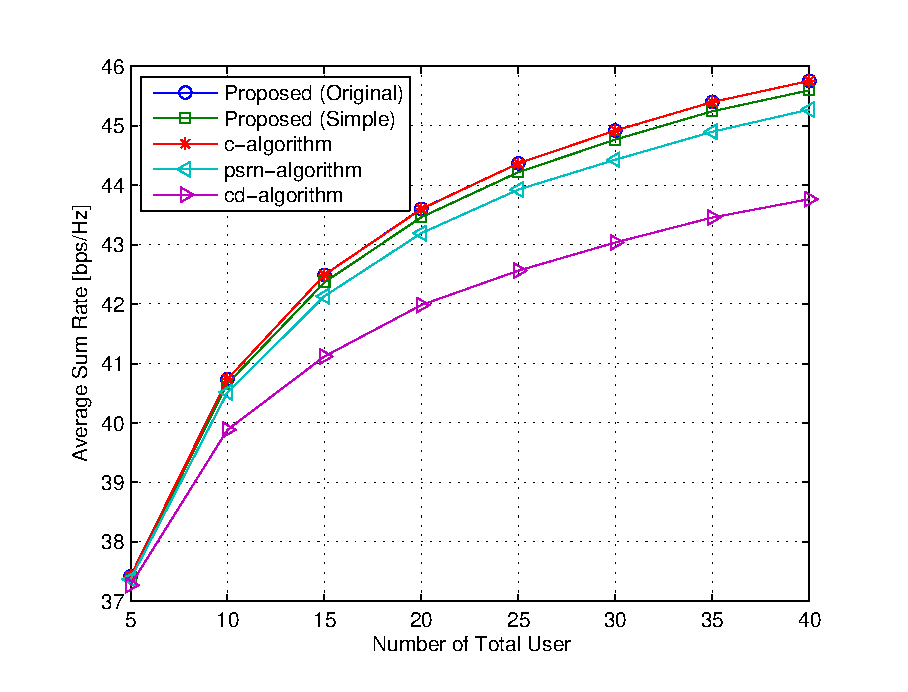
\includegraphics[width=0.50\textwidth]{SNR20dB.eps}
\caption{Average sum rate comparison of various user selection algorithms when $n_t=8, n_r=2,$ SNR = 20 dB}  \label{Figure:SumRate1}
\end{figure}

\begin{figure}[!tb]
    \centering
    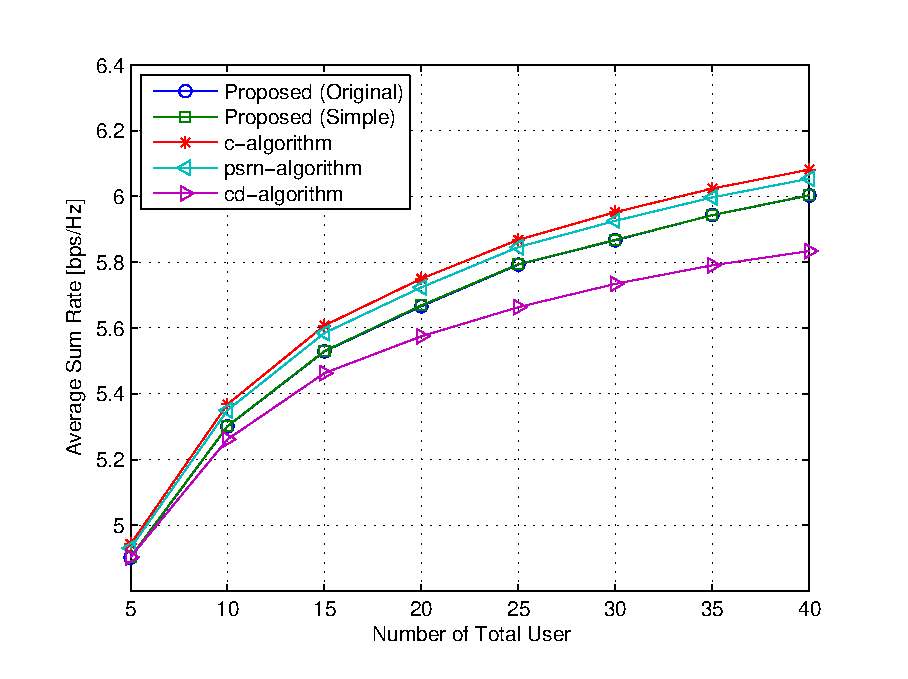
\includegraphics[width=0.50\textwidth]{SNR0dB.eps}
\caption{Average sum rate comparison of various user selection algorithms when $n_t=8, n_r=2,$ SNR = 0 dB}  \label{Figure:SumRate2}
\end{figure}

Fig. \ref{Figure:SumRate1} and \ref{Figure:SumRate2} show the average sum rate of various scheduling algorithms versus the number of total users $\hat{K}$ with fixed $n_t=8$, $n_r=2$ when SNR = 20 dB and SNR = 0 dB, respectively \cite{SRN}. As seen in the Figures, c-algorithm outperforms other methods, because the user selection metric is direct sum rate of BD. In Fig \ref{Figure:SumRate1}, the proposed algorithm has almost the same performance with c-algorithm at SNR = 20 dB. The reason is that the selection metric represents the data rate of BD in high SNR regime. We can notice that the proposed algorithm outperforms both the psrn-algorithm and cd-algorithm of the similar complexity order with the proposed algorithm. However, in low SNR regime (for the case SNR = 0 dB), the sum rate of the proposed algorithm is slightly lower than that of psrn-algorithm. The proposed selection metric does not indicate data rate of BD in low SNR regime. Nonetheless, the proposed algorithm provides better performance than cd-algorithm, and can achieves 99$\%$ sum rate of c-algorithm.

In addition, we figure out the performance gap between original metric and simplified metric of the proposed algorithm. In low SNR regime, loss from the simplified metric is negligible. In high SNR regime, the sum rate loss from the simplified metric is only about 0.35\%, and it still achieves the 99\% sum rate of c-algorithm and performs better than psrn-algorithm and cd-algorithm.

\begin{figure}[!tb]
    \centering
    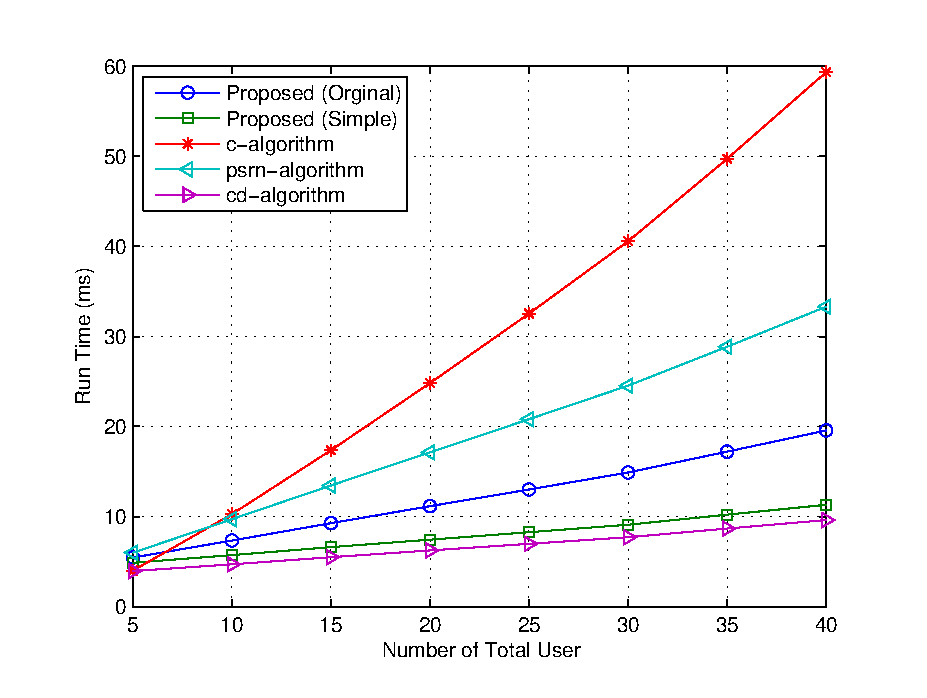
\includegraphics[width=0.50\textwidth]{RunTime.eps}
\caption{Run time comparison of various user selection algorithms when $n_t=8, n_r=2$}  \label{Figure:RunTime}
\end{figure}

Fig. \ref{Figure:RunTime} plots CPU rum time comparison of various user selection algorithms when $n_t=8, n_r=2$. These results obtained by 2.26 GHz Core2Duo CPU PC. It is observed that the proposed algorithm with the simplified metric has similar run time with cd-algorithm which has the shortest run time. However, the proposed algorithm with the simplified metric has almost the same performance as c-algorithm as seen in Fig \ref{Figure:SumRate1} and \ref{Figure:SumRate2}. Thus, it can be said that the simplified metric can reduce the complexity greatly with negligible throughput loss.

\begin{figure}[!tb]
    \centering
    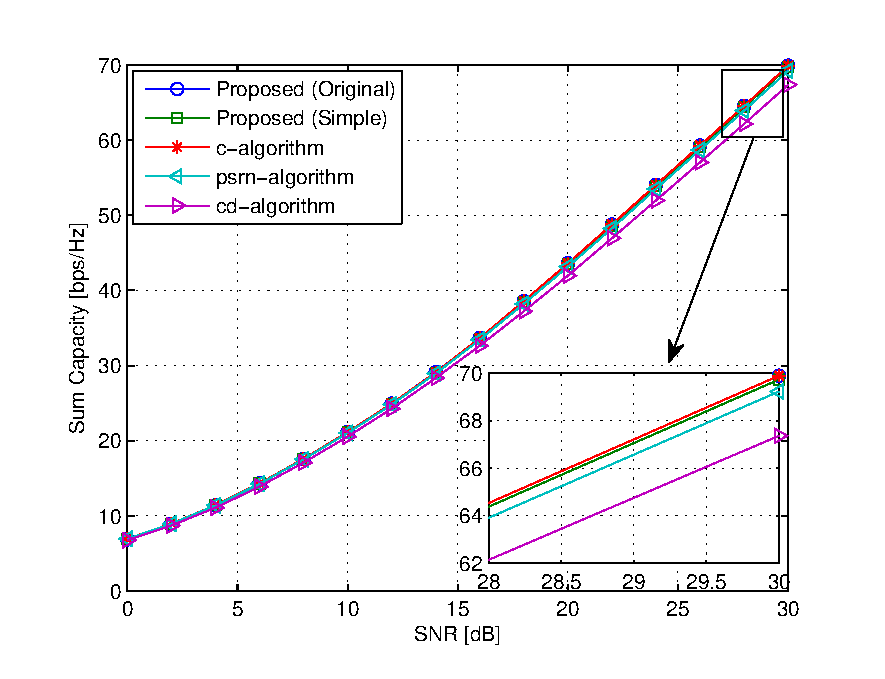
\includegraphics[width=0.50\textwidth]{RateVSSNR.eps}
\caption{Average sum rate versus SNR when $n_t=8, n_r=2, K = 20$}  \label{Figure:RateVSSNR}
\end{figure}

Fig. \ref{Figure:RateVSSNR} shows average sum rate versus SNR when $n_t=8, n_r=2, K = 20$. As seen in Fig. \ref{Figure:RateVSSNR}, the proposed algorithm provides better performance than psrn-algorithm in high SNR regime (from SNR = 5 dB). In high SNR regime, the performance gap between the proposed algorithm and other algorithms becomes much larger. As the SNR gets higher, the performance of other algorithms gets lower because their selection metric does not represent rate in high SNR regime.

\begin{figure}[!tb]
    \centering
    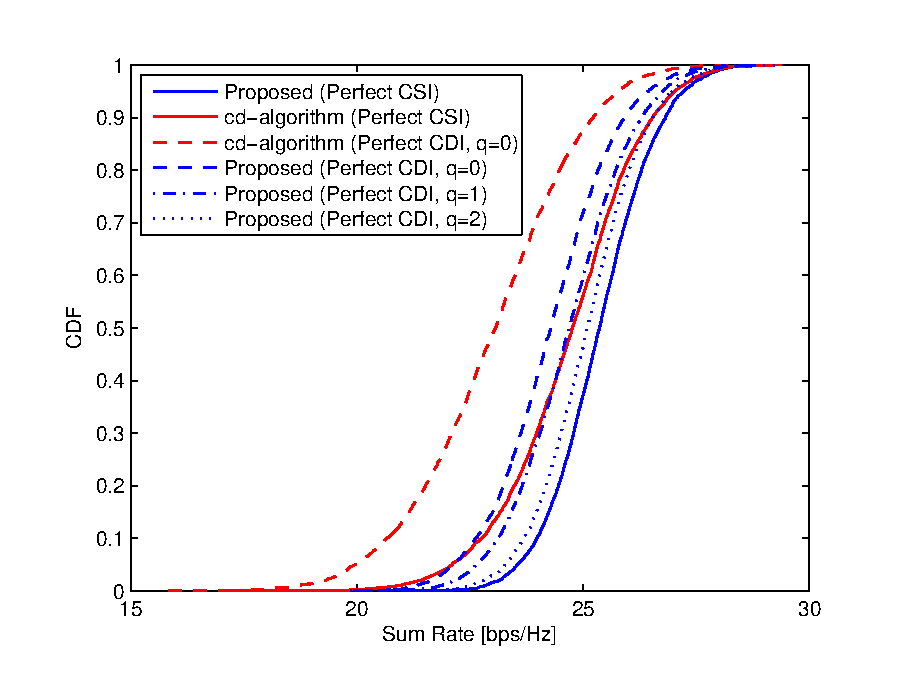
\includegraphics[width=0.50\textwidth]{CDF_fullCDI20dB.eps}
\caption{Empirical CDF of average sum rate when $n_t=4, n_r=2, K=20$ SNR $= 20$ dB, where the BS has perfect direction information and imperfect quality information.}  \label{Figure:FullCDI}
\end{figure}

\begin{figure}[!tb]
    \centering
    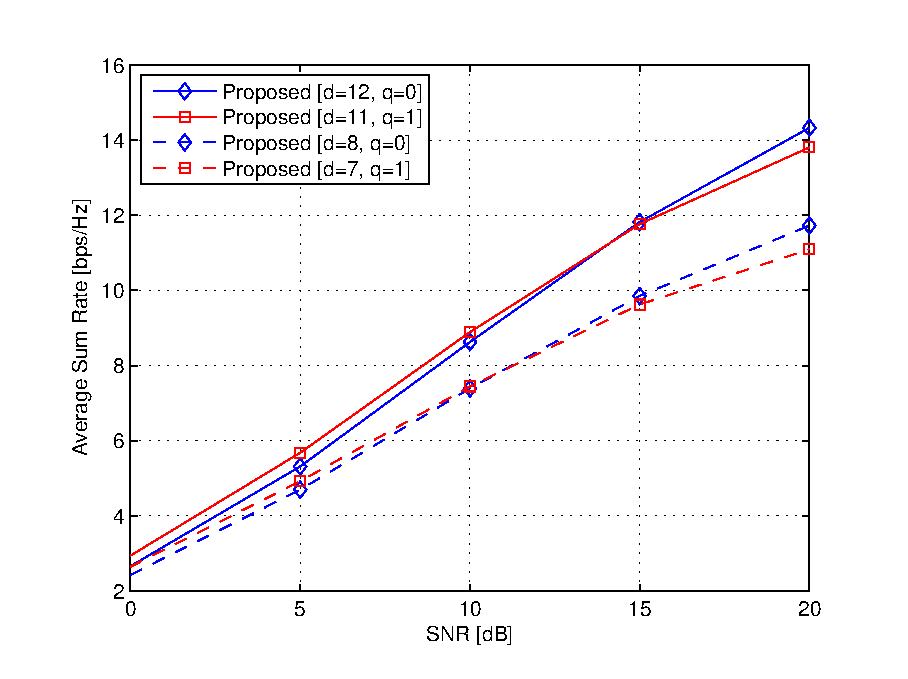
\includegraphics[width=0.50\textwidth]{12_8bits.eps}
\caption{Average sum rate versus SNR when $n_t=4, n_r=2, K = 20$, where the BS has imperfect direction information and quality information.}  \label{Figure:PartialCDI}
\end{figure}

Fig. \ref{Figure:FullCDI} and \ref{Figure:PartialCDI} show the performance comparison in limited feedback systems where a BS has the imperfect CSI. In Fig. \ref{Figure:FullCDI}, we assume that the BS has perfect direction information and quantized channel quality information. Specifically, the row basis of channel matrix is explicitly fed back to the BS and the quantized determinant of effective channels is fed back to the BS. In this simulation, inter-user interference can be completely eliminated since direction information is perfectly known at the BS. Thus, Fig. \ref{Figure:FullCDI} shows the only user selection performance according to the amount of quality information feedback. For comparison, we also provided the performance of cd-algorithm which selects a user set using only direction information. As seen in Fig. \ref{Figure:FullCDI}, 1 bit quality information are enough to achieve the sum rate of cd-algorithm with perfect CSI. Thus, we can conclude that channel quality information feedback makes the BS select a good user set even if feedback amount is very small.

In Fig. \ref{Figure:PartialCDI}, we consider a limited feedback system with quantized direction information and quality information. The rest of simulation setup is the same as in Fig. \ref{Figure:FullCDI}. We assume the case when the total feedback amounts are 12 bits and 8 bits. In this scenario, a precoder cannot be designed perfectly to eliminate inter-user interference, because the BS does not know perfect direction information, which causes throughput decrease. As seen in Fig. \ref{Figure:PartialCDI}, in low SNR regime, quality information feedback gives throughput gain, but in high SNR regime, it does not. Specifically, 1 bit quality information feedback brings about 10\% throughput gain compared to the case without quality information feedback when SNR = 0 dB. The reason is as follows. In high SNR regime, interference is dominant over noise power so channel direction information is more important than quality information for designing a precoder. In other words, although a user set is well-selected by the proposed user selection algorithm with quality information feedback, the data rate is decreased due to an ill-designed precoder. On the other hands, in low SNR regime, where noise power is dominant so that quality information feedback causes significant throughput gain from the well-selected user set.

\begin{figure}[!tb]
    \centering
    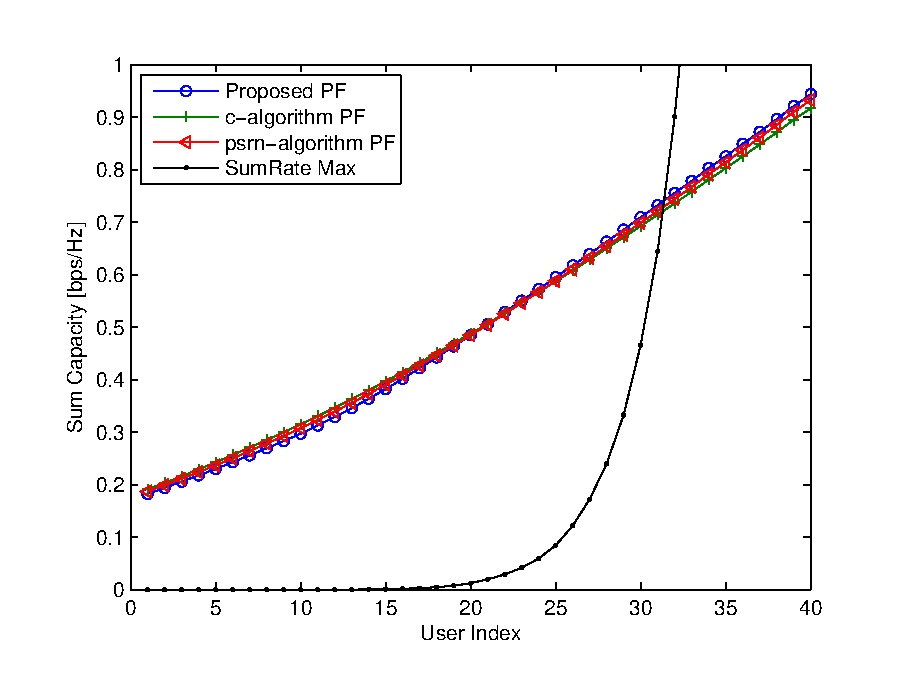
\includegraphics[width=0.50\textwidth]{PF2.eps}
\caption{Average rate of individual users}  \label{Figure:PF}
\end{figure}

For the performance of PF scheduling, the individual data rate of users for unequal SNRs is provided in Fig \ref{Figure:PF}. In simulation runs, we fix the total number of users $K$ by 40 and the number of antennas, $n_t=8$ and $n_r=2$, respectively. And the SNR of users ranges from 0 dB to 20 dB \cite{SimulationPF}. More specifically, SNR  increases linearly as the index of user increases (i.e., the SNR of the first index user and the last index user is 0 dB and 20 dB, respectively). As shown in Fig. \ref{Figure:PF}, the proposed PF algorithm provides almost the same performance as PF c-algorithm. It can be observed that the proposed PF algorithm slightly favors the users with a high SNR.


\section{Conclusion} \label{Section:Conclustion}
In this paper, we propose a greedy user selection algorithm, where the product of eigenvalues of effective channel matrices is used as the selection metric at each iteration. The idea is motivated by the fact that the data rate is closely related to the eigenvalues of effective channel matrix. The key contributions of this paper are as follows: First, we show the product of eigenvalues can be obtained recursively from the previous iteration using relationship between eigenvalues and principal angles; Secondly, we find the lower bound of the product of eigenvalues, which is utilized as a simple selection metric in our proposed algorithm. In this way, we can reduce complexity significantly. Lastly we show that  the proposed scheme is directly applicable to PF scheduling since the selection metric is based on the sum rate of BD. Furthermore, we extend the proposed algorithm to limited feedback systems. From computational complexity analysis and simulation results, it is observed  that the proposed algorithm provides better performance than other greedy algorithms of similar complexity. Especially the proposed algorithm performs almost the same as c-algorithm in high SNR regime.

%Further work can extend the case when different numbers of antennas are adopted by users. Also, systematic effects from the lack of CSI knowledge in limited feedback systems is also left for the further work.%




% if have a single appendix:
%\appendix[Proof of the Zonklar Equations]
% or
%\appendix  % for no appendix heading
% do not use \section anymore after \appendix, only \section*
% is possibly needed

% use appendices with more than one appendix
% then use \section to start each appendix
% you must declare a \section before using any
% \subsection or using \label (\appendices by itself
% starts a section numbered zero.)
%


\appendices
\section{Proof of Theorem \ref{thm:relationship}} \label{Appendix:thm1}
The effective channel matrix of user $k$ at ($i-1$)-th iteration can be decomposed by SVD as follows:
\begin{eqnarray}
{{{\bf{\bar H}}}_k^{(i-1)}} & = & {\bar{\bf{U}}_k}[{\bar{\bf{\Sigma }}_k} \, {\bf{0}}]{[\bar{\bf{V}}_k^{(1)} \, \bar{\bf{V}}_k^{(0)}]^*} \nonumber \\
& = & {\bar{\bf{U}}_k}{\bar{\bf{\Sigma }}_k} \bar{\bf{V}}_k^{(1)*} \nonumber \\
& = & {\bar{\bf{U}}_k}{\bar{\bf{\Sigma }}_k}{\bf{B}}_k^{(i-1)*}. \label{eq:HeffPrv}
\end{eqnarray}
The third equality comes from the fact that ${\bf{B}}_k^{(i-1)}=\bar{\bf{V}}_k^{(1)}$ as in section \ref{Section:SystemModel}.

At the $i$-th iteration, the effective channel matrix of user $k$ is expressed as follows:
\begin{eqnarray}
{{{\bf{\bar H}}}_k^{(i)}} & = & {{{\bf{\bar H}}}_k^{(i-1)}}{\bf{G}}_k^{(i)} \nonumber \\
& = & {\bar{\bf{U}}_k}{\bar{\bf{\Sigma }}_k}{\bf{B}}_k^{(i-1)*}{{\bf{G}}_k^{(i)}} \label{eq:HeffNext},
\end{eqnarray}
where (\ref{eq:HeffNext}) is obtained by substituting ${{\bf{\bar H}}}_k^{(i-1)}$ to (\ref{eq:HeffPrv}). Then the product of eigenvalues of ${{{\bf{\bar H}}}_k^{(i)}}{{{\bf{\bar H}}}_k^{(i)*}}$ is given by
\begin{eqnarray}
\mu _k^{(i)} & = & \det \left({\bf{\bar H}}_k^{(i)}{\bf{\bar H}}_k^{(i)*}\right) \nonumber \\
& = & \det \left({\bar{\bf{U}}_k}{\bar{\bf{\Sigma }}_k}{\bf{B}}_k^{(i-1)*}{{\bf{G}}_k^{(i)}}{{\bf{G}}_k^{(i)*}}{\bf{B}}_k^{(i-1)}{\bar{\bf{\Sigma }}_k^*}\bar{\bf{U}}_k^*\right) \label{eq:Appendixmu1} \nonumber \\
% & = &\det ({{\bf{U}}_p})\det ({{\bf{D}}_p})\det ({\bf{V}}_p^{(1)*}{\bf{G}}{{\bf{G}}^*}{\bf{V}}_p^{(1)})\det ({\bf{D}}_p^*)\det ({\bf{U}}_p^*)\\
& = & \mu _k^{(i-1)}\det \left({\bf{B}}_k^{(i-1)*}{{\bf{G}}_k^{(i)}}{{\bf{G}}_k^{(i)*}}{\bf{B}}_k^{(i-1)}\right). \label{eq:Appendixmu2}
\end{eqnarray}
The last equality can be obtained by the following: Because ${\bar{\bf{\Sigma }}_k}$ is diagonal matrix whose diagonal entries are singular values of ${{\bf{\bar H}}}_k^{(i-1)}$, $\det({\bar{\bf{\Sigma }}_k})\det({\bar{\bf{\Sigma }}_k}^*)=\mu _k^{(i-1)}$, and $\det(\bar{\bf{U}}_k)\det(\bar{\bf{U}}_k^*)=1$ since $\bar{\bf{U}}_k$ is unitary matrix.

As seen in Section \ref{Section:SystemModel}, ${\bf{B}}_k^{(i-1)}$ and ${\bf{G}}_k^{(i)}$ represent $\mathrm{row}\left({{\bf{H}}_k}{\bf{Z}}_k^{(i-1)}\right)$ and  $\mathrm{null}\left({{\bf{H}}_{u_{i}}}{\bf{Z}}_k^{(i-1)}\right)$, respectively, where ${u_{i}}$ denotes the selected user at the $i$-th iteration. So, from the relationship between principal angles and eigenvalues,
\begin{equation}
\det \left({\bf{B}}_k^{(i-1)*}{{\bf{G}}_k^{(i)}}{{\bf{G}}_k^{(i)*}}{\bf{B}}_k^{(i-1)}\right) = \prod\limits_{l=1}^{{n_r}} {\cos^2 {\theta_{k,l}}},
\end{equation}
where $\{\theta_{k,l}\}_{l=1}^{n_r}$ represents principal angles between ${\cal{R}}\left({{\bf{H}}_k}{\bf{Z}}_k^{(i-1)}\right)$ and ${\cal{N}}\left({{\bf{H}}_{u_{i}}}{\bf{Z}}_k^{(i-1)}\right)$. Let $\phi_k$ denote the product angles between ${\cal{R}}\left({{\bf{H}}_k}{\bf{Z}}_k^{(i-1)}\right)$ and ${\cal{N}}\left({{\bf{H}}_{u_{i}}}{\bf{Z}}_k^{(i-1)}\right)$, i.e.,
\begin{eqnarray} \label{eq:ProdAngle}
\cos ^2 \phi_k & = & \cos ^2 \measuredangle \left({\cal{R}}\left({{\bf{H}}_k}{\bf{Z}}_k^{(i-1)}\right), {\cal{N}}\left({{\bf{H}}_{u_{i}}}{\bf{Z}}_k^{(i-1)}\right)\right) \nonumber \\
& = & \prod\limits_{l=1}^{{n_r}} {\cos ^2 {\theta_{k,l}}}.
\end{eqnarray}

Then, (\ref{eq:Appendixmu2}) can be rewritten as
\begin{equation} \label{eq:Appendixmu3}
\mu _k^{(i)} = \mu _k^{(i-1)}{\cos^2 \phi_k},
\end{equation}
which completes the proof.

\section{Proof of Theorem \ref{thm:lowerbound}} \label{Appendix:thm2}
Originally, $\phi_k$ is defined by the product angle between ${\cal{R}}\left({{\bf{H}}_k}{\bf{Z}}_k^{(i-1)}\right)$ and ${\cal{N}}\left({{\bf{H}}_{u_{i}}}{\bf{Z}}_k^{(i-1)}\right)$. By the property that the principal angles between subspaces is the same as those between their orthogonal complements \cite{AngleOrthogonal, AngleOrthogonal2}, $\cos \phi_k$ is the same as the product angles between  ${\cal{N}}\left({{\bf{H}}_k}{\bf{Z}}_k^{(i-1)}\right)$ and ${\cal{R}}\left({{\bf{H}}_{u_{i}}}{\bf{Z}}_k^{(i-1)}\right)$. Given two matrices ${\bf{A}}$ and ${\bf{B}}$ with $\textrm{rank}({\bf{A}}) \leq \textrm{rank}({\bf{B}})$, the product angle between ${\cal{R}}(\bf{A})$ and ${\cal{C}}(\bf{B})$ is alternatively defined as \cite{ProductAngle2}
\begin{equation}
\cos ^2 \measuredangle (\cal{R}({\bf{A}}),\cal{C}({\bf{B}}) )=\frac{\det({\bf{A}}{\bf{B}}{\bf{B}}^*{\bf{A}}^*)} {\det({\bf{A}}{\bf{A}}^*)},
\end{equation}
where ${\cal{C}}(\bf{B})$ denotes the column space of matrix $\bf{B}$.

Let $\bf{W}$ be ${\bf{Z}}_k^{(i-1)} \times \mathrm{null}\left({{\bf{H}}_k}{\bf{Z}}_k^{(i-1)}\right)$. Note that $\bf{W}$ lies in the null space of selected users' channel matrices.

Then, $\cos^2 \phi_k$ is given by
\begin{eqnarray}
\cos^2 \phi_k & = & \frac {\det \left( {\bf{H}}_{u_{i}} {\bf{W}} {\bf{W}}^* {\bf{H}}^*_{u_{i}}\right)} {\det\left({{\bf{H}}_{u_{i}}}{\bf{Z}}_k^{(i-1)} {\bf{Z}}_k^{(i-1)*}{\bf{H}}_{u_{i}}^*\right)} \nonumber \\
& = & \frac {\det \left( {\bf{H}}_{u_{i}} {\bf{W}} {\bf{W}}^* {\bf{H}}_{u_{i}}\right) / \det \left( {\bf{H}}_{u_{i}} {\bf{H}}^*_{u_{i}}\right) }
 {\det\left({{\bf{H}}_{u_{i}}}{\bf{Z}}_k^{(i-1)} {\bf{Z}}_k^{(i-1)*}{\bf{H}}_{u_{i}}^*\right) / \det \left( {\bf{H}}_{u_{i}} {\bf{H}}^*_{u_{i}}\right)} \nonumber \\
%& = & \frac{\det ( {\bf{O}}_{u_{i}}^* {\bf{W}} {\bf{W}}^* {\bf{O}}_{u_{i}})} { \det({{\bf{O}}_{u_{i}}^*}{\bf{Z}}_k^{(i-1)} {\bf{Z}}_k^{(i-1)*}{{\bf{O}}_{u_{i}}})} \nonumber \\
& = & \frac{\cos^2 \varphi_{{u_i}, s}} {\cos^2 \varphi_{{u_i}, s \setminus k }},
\end{eqnarray}
where $\varphi_{{u_i}, s} = \measuredangle \left({\cal{R}}\left({{\bf{H}}_{u_i}}\right), {\cal{N}}\left({{\bf{H}}_{s}} \right)\right)$ and $\varphi_{{u_i}, s \setminus k } = \measuredangle \left({\cal{R}}\left({{\bf{H}}_{u_i}}\right), {\cal{N}}\left({{\bf{H}}_{s \setminus k}} \right)\right)$.

This completes the proof.

\bibliographystyle{IEEEtran}
\bibliography{IEEEabrv,MUMIMO}



% biography section
%
% If you have an EPS/PDF photo (graphicx package needed) extra braces are
% needed around the contents of the optional argument to biography to prevent
% the LaTeX parser from getting confused when it sees the complicated
% \includegraphics command within an optional argument. (You could create
% your own custom macro containing the \includegraphics command to make things
% simpler here.)
%\begin{biography}[{\includegraphics[width=1in,height=1.25in,clip,keepaspectratio]{mshell}}]{Michael Shell}
% or if you just want to reserve a space for a photo:

\begin{biography}[{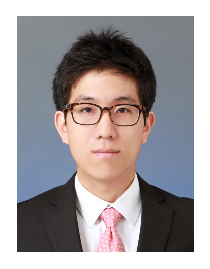
\includegraphics[width=1in,height=1.25in,clip,keepaspectratio]{seongho.eps}}]{Seongho Nam}
received the B.S degree in information and communication engineering from Inha University, Korea, in 2011, and received the M.S degree in electrical engineering from Korea Advanced Institute of Science and Technology (KAIST), Korea, in 2013. He is currently with agency for defense development (ADD), Korea. His research interest includes multi-user MIMO and cooperative communications.
\end{biography}

\begin{biography}[{\includegraphics[width=1in,height=1.25in,clip,keepaspectratio]{jeongchan.eps}}]{Jeongchan Kim}
received his B.S. degree in Electronics Engineering, from Konkuk University, Seoul, Korea, in 2006, and the M.S. in information \& Communications Engineering from Korea Advanced Institute of Science and Technology (KAIST). He is currently pursuing the Ph.D. degree in the Department of Electrical Engineering from Korea Advanced Institute of Science and Technology (KAIST). His research interests are in the areas of MIMO systems, interference management, and cooperative communications.
\end{biography}

\begin{biography}[{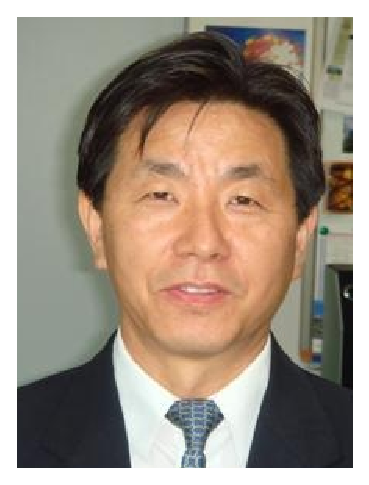
\includegraphics[width=1in,height=1.25in,clip,keepaspectratio]{youngnam.eps}}]{Youngnam Han}
received his B.S and M.S. in Electrical Engineering from Seoul National University in 1978 and 1980, respectively. He received his Ph.D. from the University of Massachusetts, Amherst in 1992. He had been working as a principal engineer at ETRI during 1992 to 1997 managing the project of design and performance analysis of radio transmission technology for DCN, PCS and IMT2000. He was actively engaged in R\&D for IS95 digital cellular system in Korea deployed nationwide in 1995 and as a member for IMT2000 standards activities as a delegate at ITU-R representing Korea. He joined ICU as a faculty since 1998, and was a principal engineer at Qualcomm, Inc. San Diego during 2001~2001, where he worked on the standards cdma20001xEV. He had been served many conferences as a TPC member and organizing chairs. And TPC chair for VTC2003 Spring. He had been a Chairman of BoG, IEEE VTS APWCS (Asia Pacific Wireless Communication Symposium) during 2009~2010. He will serve as a general chair for VTC2014 Spring in Seoul. He is currently with the Department of Electrical Engineering at KAIST as a Professor. His research interests include performance evaluation of mobile communication systems, radio resource management, optimization of mobile systems operations and cognitive radio systems. He is a recipient of a best paper Award in IEEE VTC2000, Tokyo. He is a life-long member of KICS, and a senior member of IEEE. Since June 2013, He has been working as Chair, Steering Committee, 5G Forum in Korea.
\end{biography}




\end{document}

